\documentclass{beamer}

\usetheme{Madrid}
\usecolortheme{lily}

\usepackage[utf8]{inputenc}
\usepackage{graphicx}
\usepackage{booktabs}
\usepackage{hyperref}
\usepackage{multicol}
\usepackage{array}
\usepackage{xcolor}

\bibliographystyle{unsrt}

\title{Semantic Textual Similarity}
\subtitle{IHLT Project}
\author{Oriol Miró \& Niklas Long}
\institute{MAI | UPC}
% \date{\today}

\begin{document}

% Slide 1: Introduction
\begin{frame}
  \titlepage
\end{frame}

% Slide 2: Index
\begin{frame}
  \frametitle{Outline}
  \tableofcontents
\end{frame}

\section{Methodology}

% Slide 3: Approaches Based on UKP and TakeLab
\begin{frame}
  \frametitle{1. Our Approach: UKP\cite{bar-etal-2012-ukp} and TakeLab\cite{saric-etal-2012-takelab}}
  \begin{itemize}
    \item \textbf{UKP Team:}
    \begin{itemize}
      \item Focused on extensive feature engineering.
      \item Leveraged resources like WordNet, ESA, and back-translation.
      \item Emphasized semantic features and complex overlaps.
    \end{itemize}
    \vspace{0.5cm}
    \item \textbf{TakeLab Team:}
    \begin{itemize}
      \item Emphasized efficient modeling with simple yet powerful features.
      \item Utilized lexical and shallow syntactic features.
      \item Prioritized computational efficiency.
    \end{itemize}
    \vspace{0.5cm}
    \item \textbf{Our Approach:}
    \begin{itemize}
      \item Combined strengths of both teams.
      \item Integrated comprehensive feature sets across multiple dimensions.
      \item Aimed for a balance between feature richness and computational feasibility.
    \end{itemize}
  \end{itemize}
\end{frame}

% Slide 4: Features - Five Dimensions
\begin{frame}
  \frametitle{2. Features: Five Dimensions}
  \begin{center}
    \textbf{Dimensions of Features}
    \begin{itemize}
      \item \textbf{Lexical Features}: Surface-level properties (word choice and string similarities), \textbf{38 features}.
      \item \textbf{Syntactic Features}: Grammatical structures and patterns, \textbf{18 features}.
      \item \textbf{Semantic Features}: Word and sentence meanings, \textbf{28 features}.
      \item \textbf{Stylistic Features}: Writing style and tone, \textbf{3 features}.
      \item \textbf{Combined Features}: Combination of all dimensions, \textbf{87 features}
    \end{itemize}
  \end{center}
\end{frame}




% Slide 5: Fun Features to Implement
\begin{frame}
  \frametitle{3. Interesting Features Implemented}
  \begin{itemize}
    \item \textbf{Explicit Semantic Analysis (ESA):}
    \begin{itemize}
      \item Built ESA model using \textbf{300,000 Wikipedia articles}.
      \item Represented sentences in high-dimensional concept space.
      \item Computed cosine similarities between sentence representations.
    \end{itemize}
    \vspace{0.5cm}
    \item \textbf{Lexical Substitutions:}
    \begin{itemize}
      \item Enriched sentences with synonyms from WordNet.
      \item Improved matching opportunities between sentences.
    \end{itemize}
    \vspace{0.5cm}
    \item \textbf{SMT Back-Translation:}
    \begin{itemize}
      \item Translated sentences to and from intermediate languages (e.g., German, Spanish, Dutch).
      \item Generated paraphrases to enhance similarity matching.
    \end{itemize}
  \end{itemize}
\end{frame}

% Slide 6: Feature and Model Selection Methodology
\begin{frame}
  \frametitle{4. Feature and Model Selection Methodology}
  \begin{itemize}
    \item \textbf{Data Preparation:}
    \begin{itemize}
      \item Handled missing values and outliers.
      \item Standardized features using \textit{RobustScaler}.
    \end{itemize}
    \vspace{0.5cm}
    \item \textbf{Models Explored:}
    \begin{itemize}
      \item Gradient Boosting Regressor (GBR)
      \item Random Forest Regressor (RFR)
      \item Support Vector Regressor (SVR)
    \end{itemize}
    \vspace{0.5cm}
    \item \textbf{Training Strategy:}
    \begin{itemize}
      \item 5-fold cross-validation with grid search for hyperparameters.
      \item Recursive Feature Elimination (RFE) during model training.
    \end{itemize}
  \end{itemize}
\end{frame}

\section{Results}

% Slide 7: Results per Feature Set
\begin{frame}
  \frametitle{5. Results per Feature Set}
  \begin{figure}
    \centering
    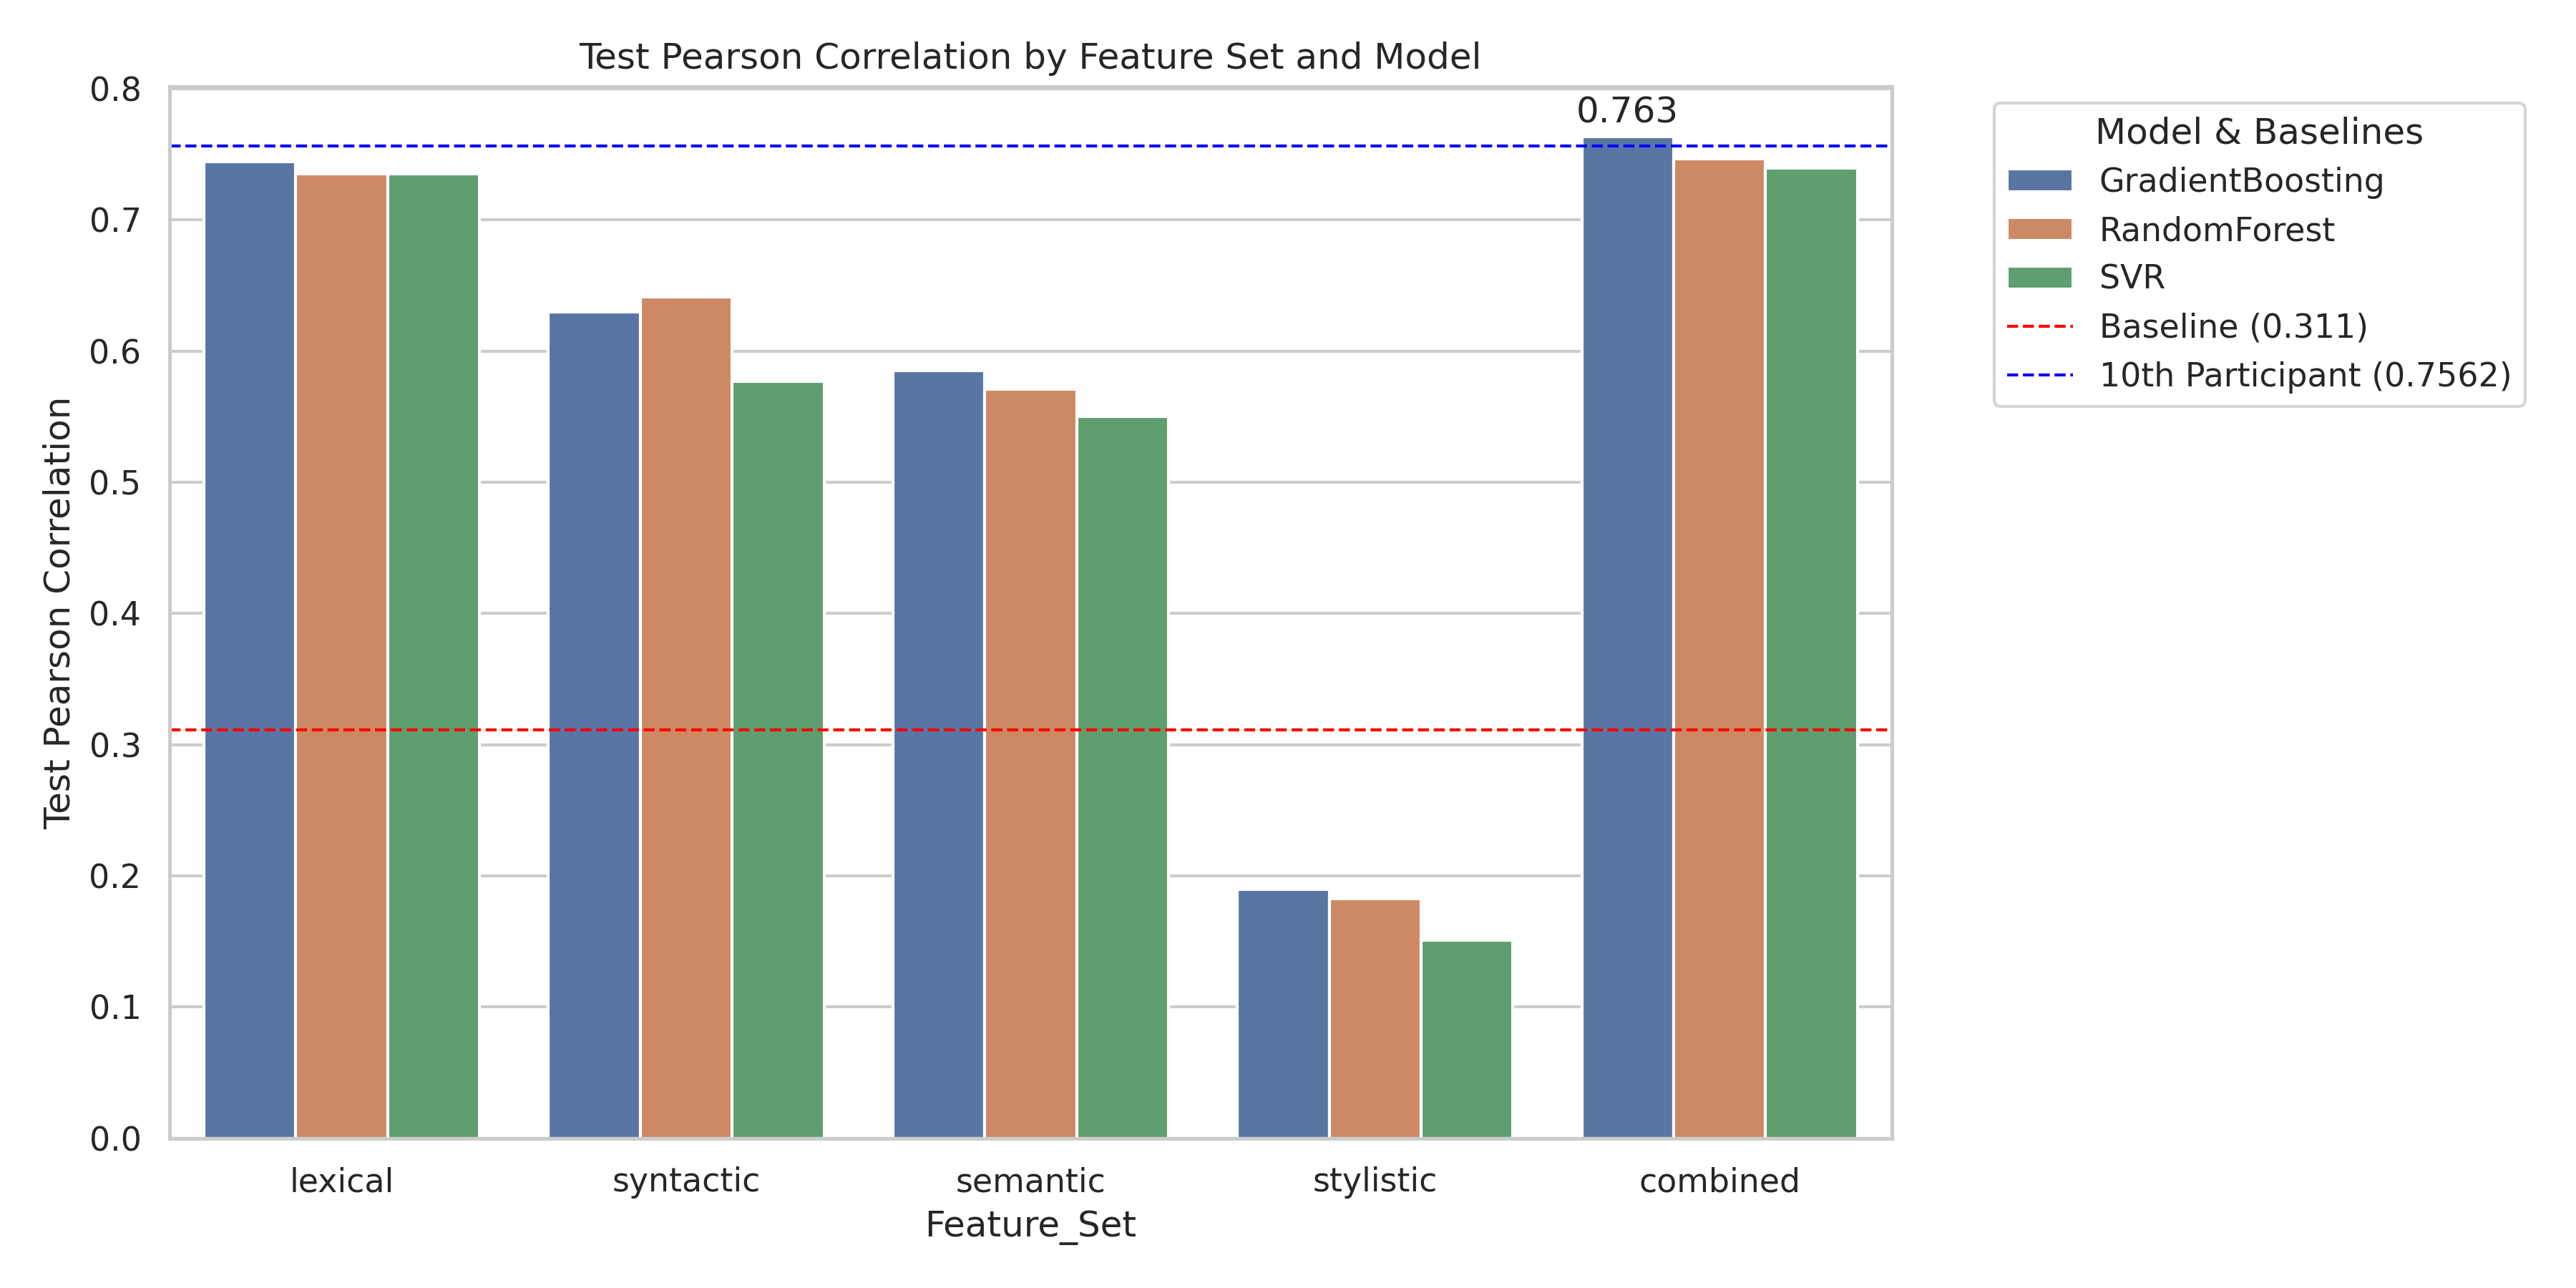
\includegraphics[width=\linewidth]{img/Test_Pearson_Correlation_by_Feature_Set_and_Model.png}
    \caption{Test Pearson Correlation by Feature Set and Model}
  \end{figure}
\end{frame}


% Slide 8: Best Results per Dataset
\begin{frame}
  \frametitle{6. Best Results per Dataset}
  \begin{itemize}
    \item Analyzed per-dataset performance for the best models.
  \end{itemize}
  \vspace{0.3cm}
  \begin{figure}
    \centering
    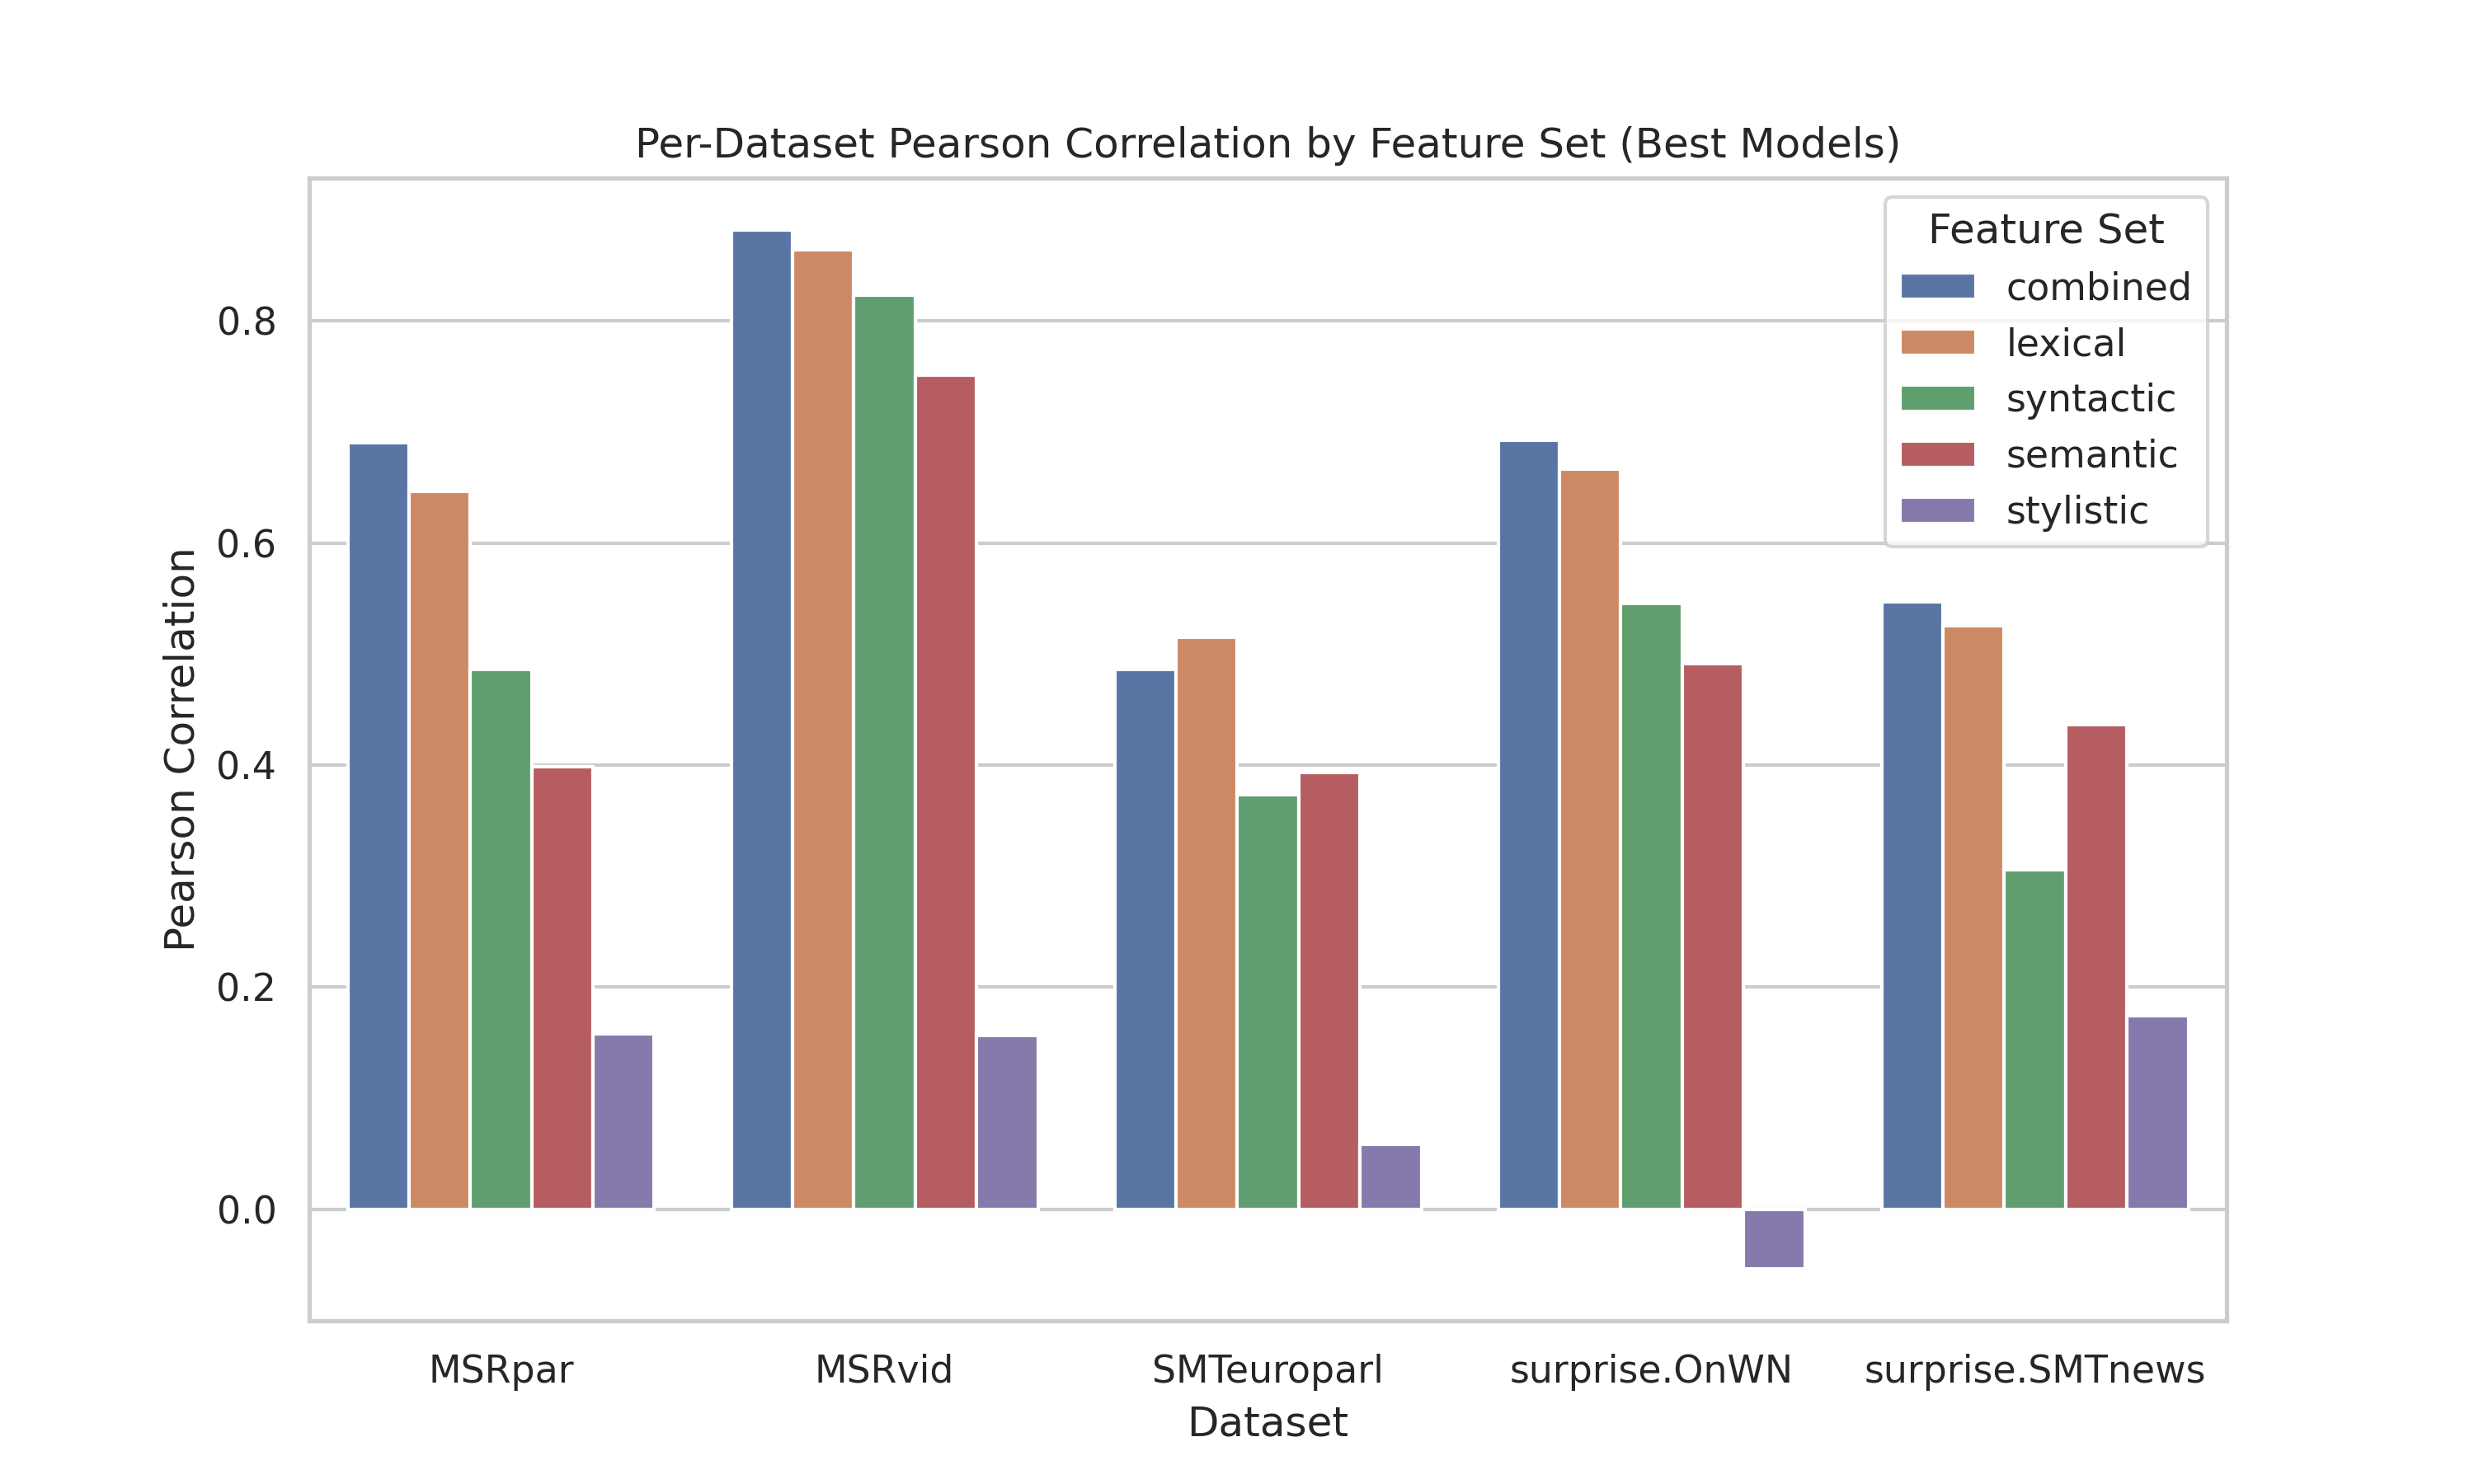
\includegraphics[width=0.85\linewidth]{img/Per-Dataset_Pearson_Correlation_by_Feature_Set_(Best_Models).png}
    \caption{Per-Dataset Pearson Correlation by Feature Set}
  \end{figure}
\end{frame}

% Slide 9: Comparison Against Competition
\begin{frame}
  \frametitle{7. Comparison Against Competition}
  \begin{itemize}
    \item Achieved an overall Pearson correlation of \textbf{0.7634}.
    \item Placed within the \textbf{top 10} in a simulated ranking.
    \item Attained the \textbf{highest mean rank}, indicating consistent performance.
  \end{itemize}
  \vspace{0.15cm}
  \begin{table}[ht]
    \centering
    \resizebox{\textwidth}{!}{%
    \begin{tabular}{>{\color{black}}lccccccccccc}
      \toprule
      \textbf{Run} & \textbf{ALL} & \textbf{Rank} & \textbf{ALLnrm} & \textbf{Rank} & \textbf{Mean} & \textbf{Rank} & \textbf{MSRpar} & \textbf{MSRvid} & \textbf{SMT-eur} & \textbf{On-WN} & \textbf{SMT-news} \\
      \midrule
      UKP-run2 & 0.8239 & 1 & 0.8579 & 2 & 0.6773 & 2 & 0.683 & 0.8739 & 0.528 & 0.6641 & 0.4937 \\
      TakeLab-syntax & 0.8138 & 2 & 0.8569 & 3 & 0.6601 & 6 & 0.6985 & 0.862 & 0.3612 & 0.7049 & 0.4683 \\
      TakeLab-simple & 0.8133 & 3 & 0.8635 & 1 & 0.6753 & 3 & 0.7343 & 0.8803 & 0.4771 & 0.6797 & 0.3989 \\
      UKP-run1 & 0.8117 & 4 & 0.8559 & 4 & 0.6708 & 5 & 0.6821 & 0.8708 & 0.5118 & 0.6649 & 0.4672 \\
      UNT-Indiv.Reg. & 0.7846 & 5 & 0.844 & 6 & 0.6162 & 14 & 0.5353 & 0.875 & 0.4203 & 0.6715 & 0.4033 \\
      ETS-PERPphr. & 0.7834 & 6 & 0.8089 & 27 & 0.6399 & 8 & 0.6397 & 0.72 & 0.485 & 0.7124 & 0.5312 \\
      ETS-PERP & 0.7808 & 7 & 0.8064 & 32 & 0.6305 & 12 & 0.6211 & 0.721 & 0.4722 & 0.708 & 0.5149 \\
      UKP-run3 & 0.779 & 8 & 0.8166 & 19 & 0.432 & 72 & 0.683 & 0.8739 & 0.528 & -0.062 & -0.052 \\
      UNT-Indiv.DT& 0.7677 & 9 & 0.8389 & 9 & 0.5947 & 26 & 0.5693 & 0.8688 & 0.4203 & 0.6491 & 0.2256 \\
      \textbf{Our Results} & \textbf{0.7634} & \textbf{10} & - & - & \textbf{0.6884} & \textbf{1} & \textbf{0.690} & \textbf{0.8817} & \textbf{0.4861} & \textbf{0.6926} & \textbf{0.5470} \\
      SRIUBC-SYS2 & 0.7562 & 11 & 0.8111 & 24 & 0.5858 & 34 & 0.605 & 0.7939 & 0.4294 & 0.5871 & 0.3366 \\
      \bottomrule
    \end{tabular}%
    }
    \caption{Table 1: Simplified names for visualisation purpose \cite{agirre-etal-2012-semeval}}
  \end{table}
\end{frame}



\section{Feature Analysis}


% Slide 10: Feature Selection
\begin{frame}
  \frametitle{8. Feature Selection}
  \begin{itemize}
    \item \textbf{Lexical Feature Set:} No features excluded.
    \item \textbf{Syntactic Feature Set:} No features excluded.
    \item \textbf{Semantic Feature Set:} 8 features excluded, including overlaps for named entities like \texttt{LAW}, \texttt{EVENT}, and \texttt{LANGUAGE}.
    \item \textbf{Stylistic Feature Set:} No features excluded.
    \item \textbf{Combined Feature Set:} No features excluded.
  \end{itemize}
  \vspace{0.5cm}
  \centering
  \textit{It was surprising that so few features were excluded.}
\end{frame}

% Slide 11: Feature Importance
\begin{frame}
  \frametitle{9. Feature Importance per model}
  \begin{figure}
    \centering
    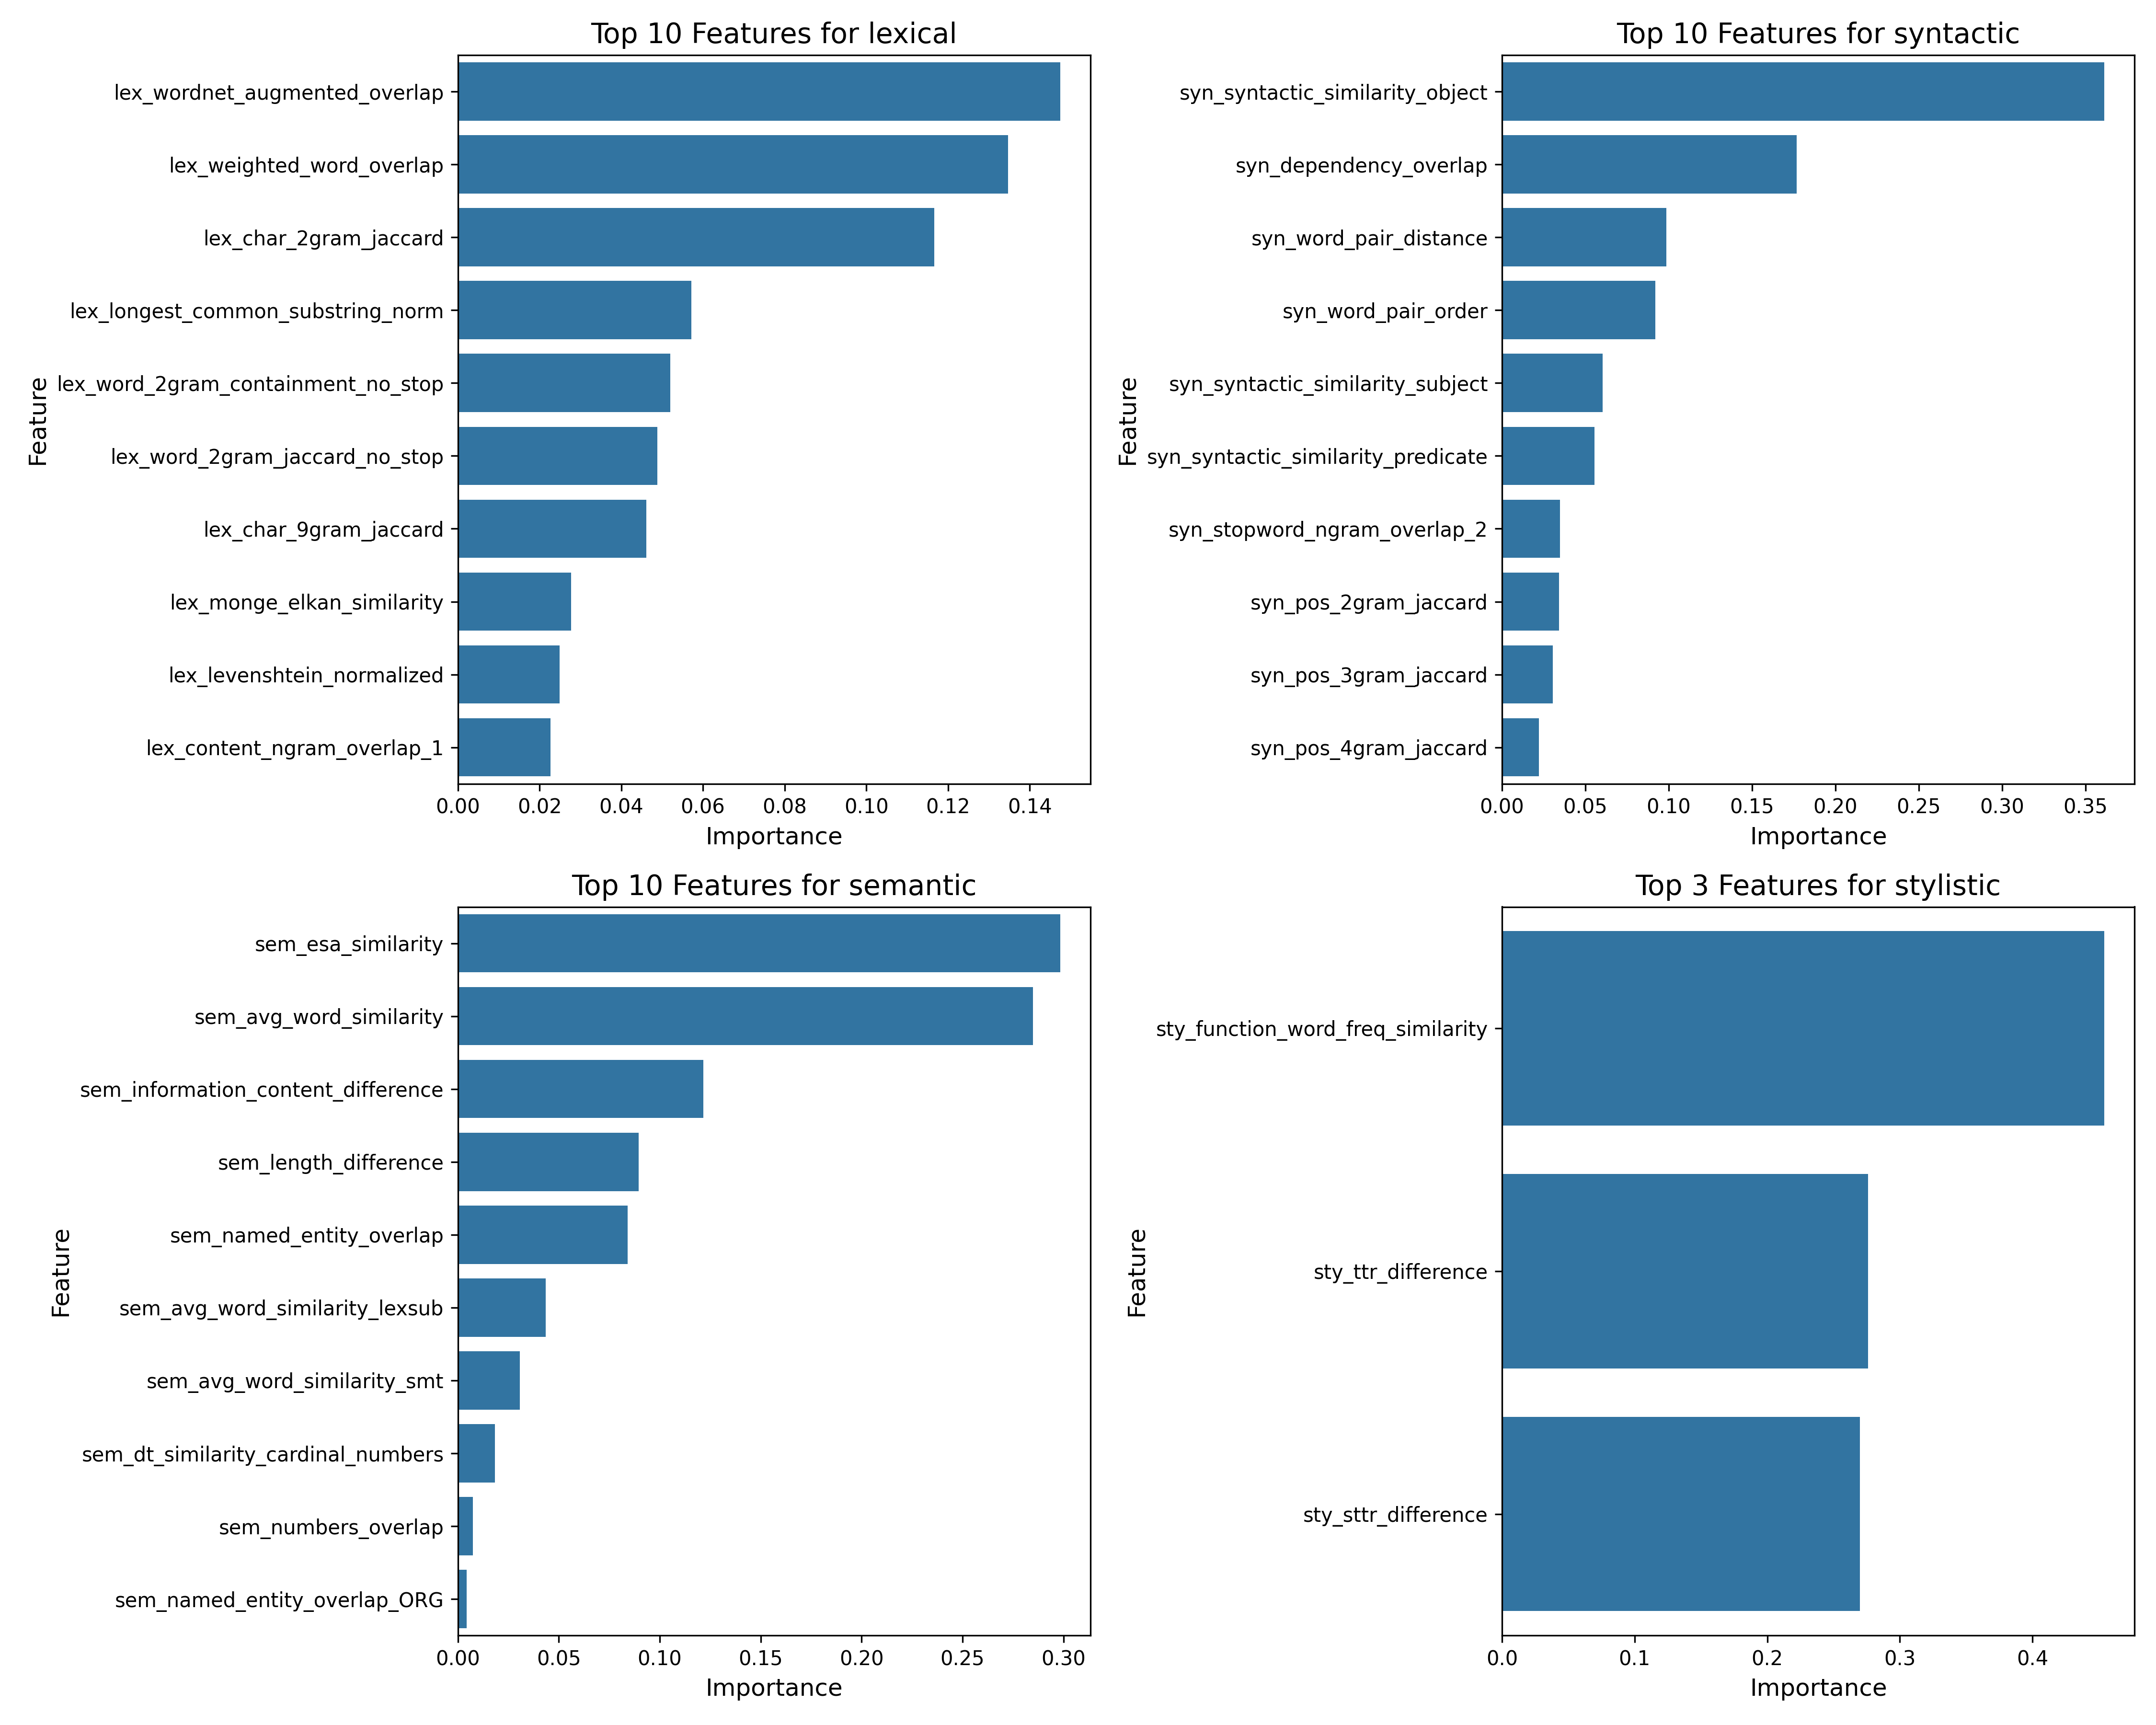
\includegraphics[width=0.7\linewidth]{img/Top_Features_Per_Feature_Set_Model.png}
    \caption{Feature Importance for All Models (bar Combined)}
  \end{figure}
\end{frame}

% Slide 12: Feature Importance Combined
\begin{frame}
  \frametitle{9. Feature Importance per model}
  \begin{figure}
    \centering
    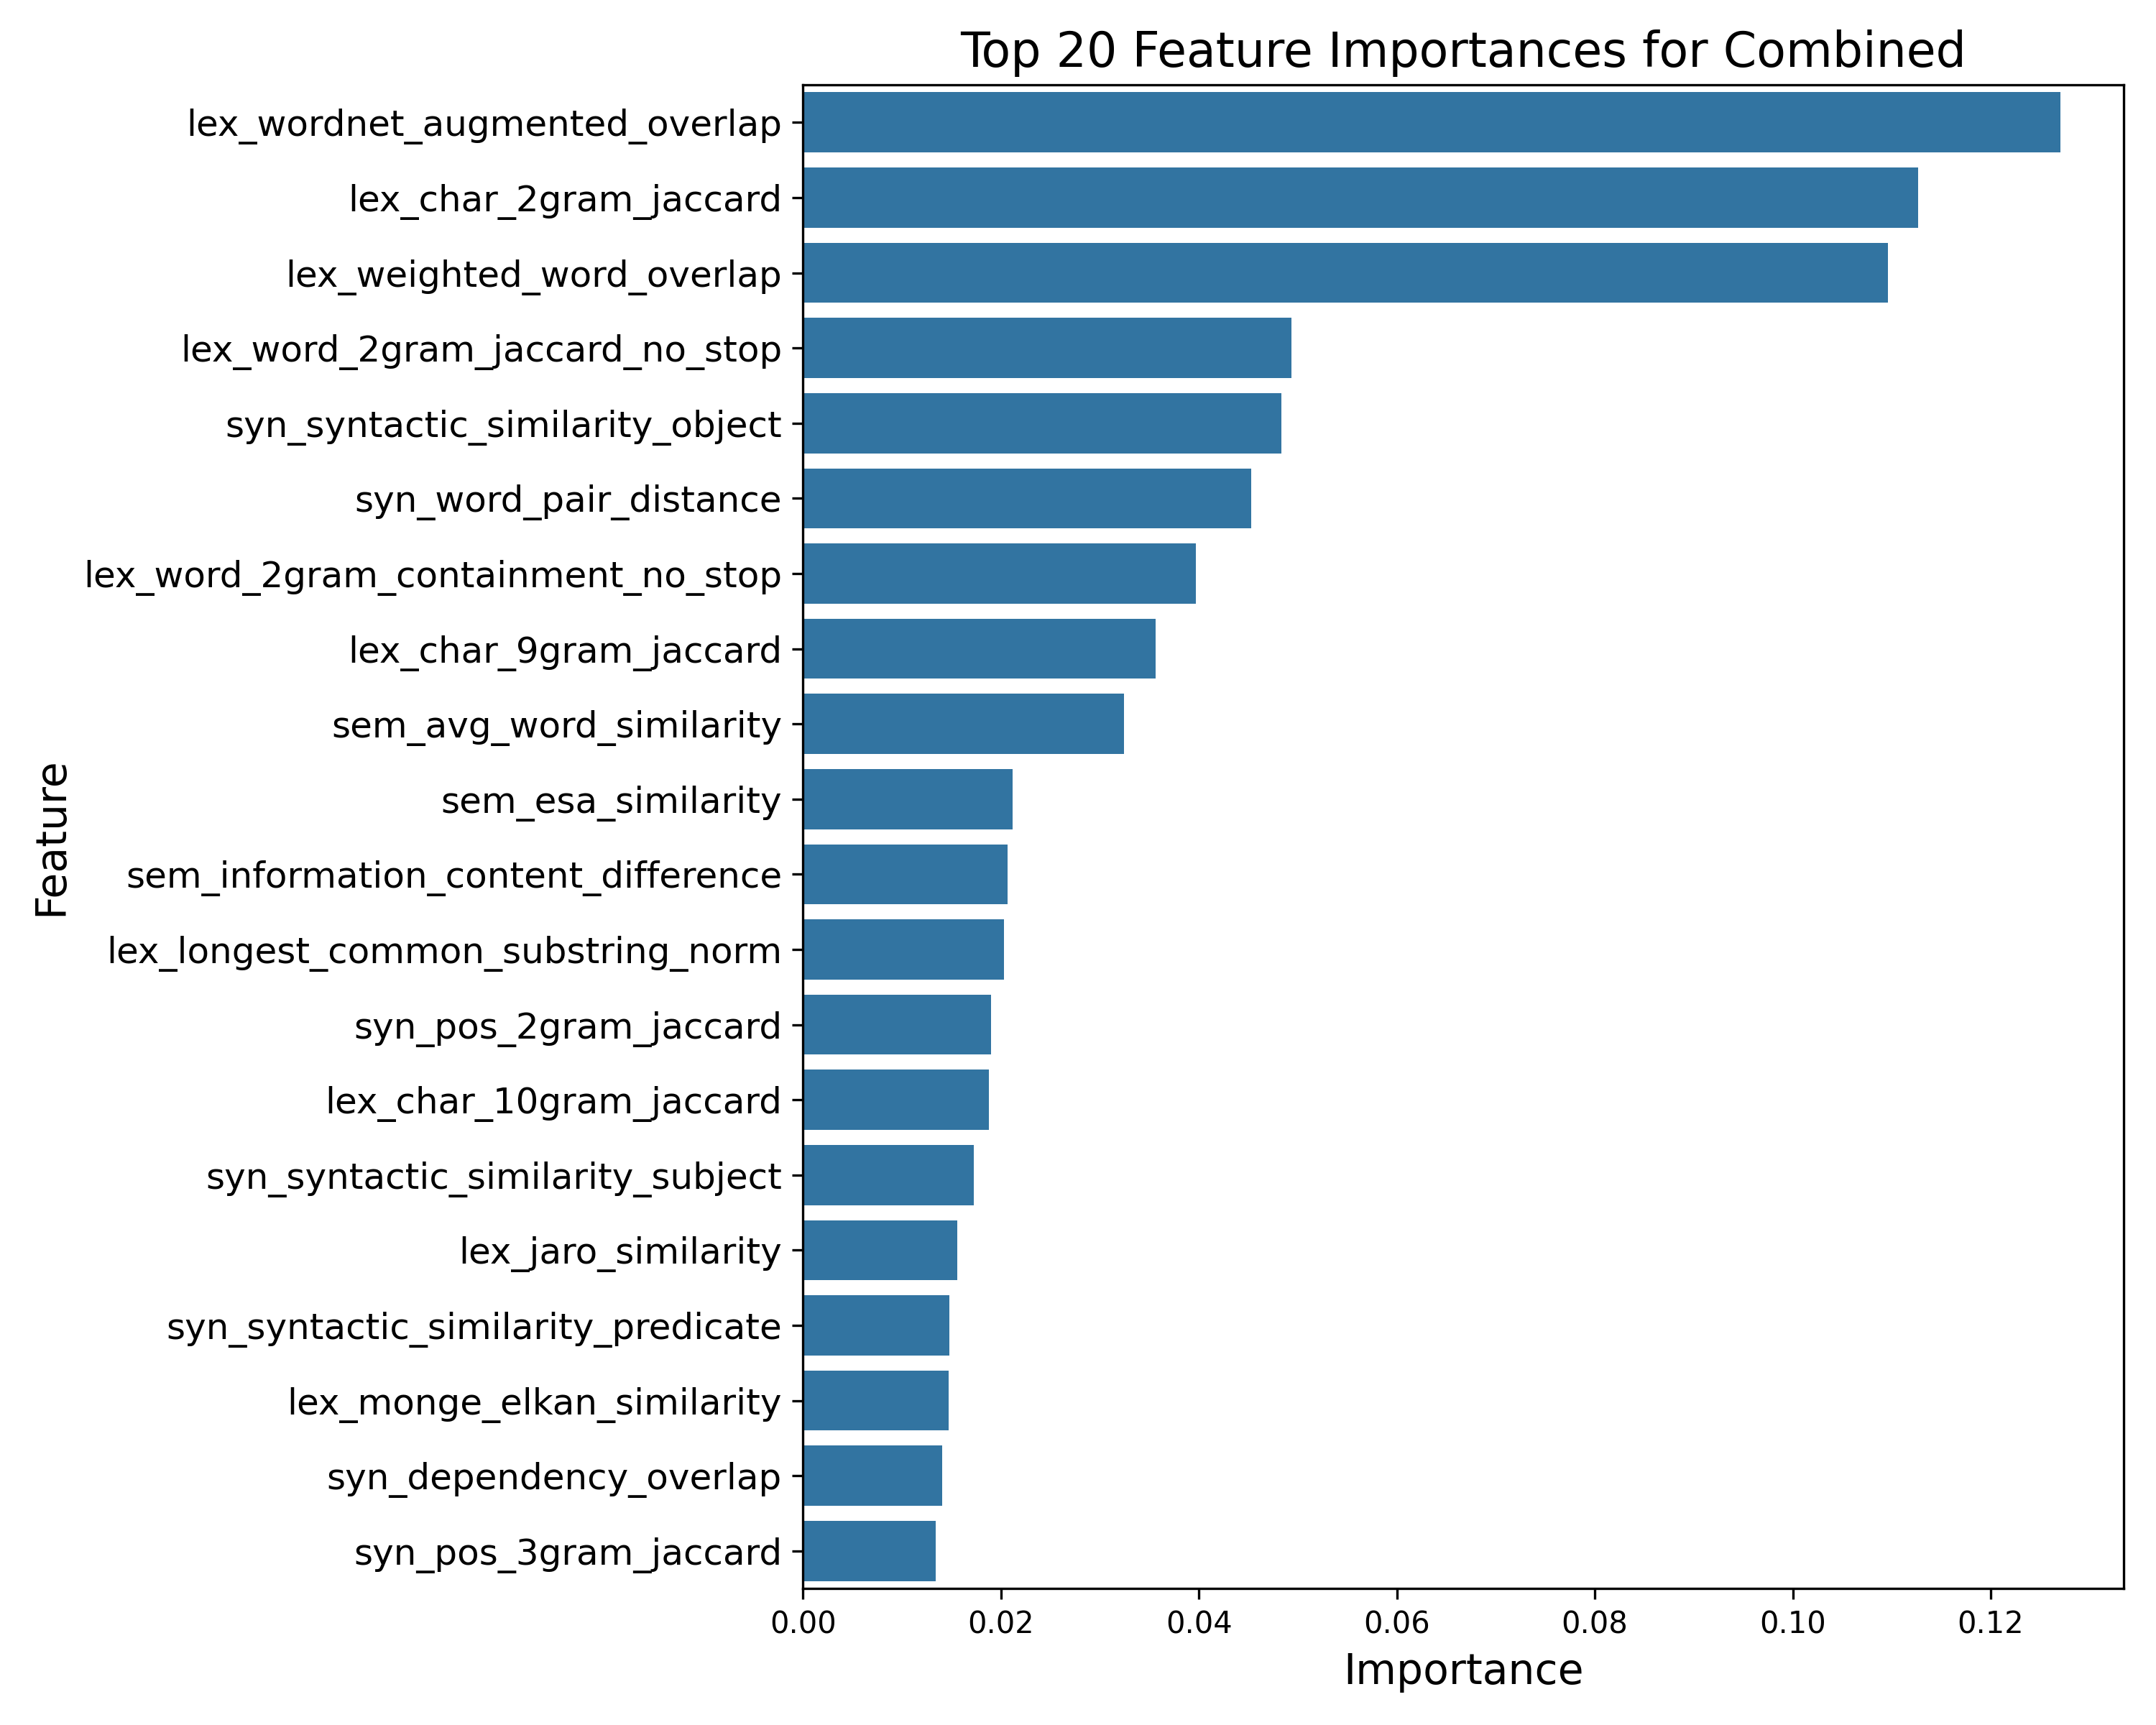
\includegraphics[width=0.7\linewidth]{img/Top_Features_Model.png}
    \caption{Feature Importance Combined Model}
  \end{figure}
\end{frame}

% Slide 13: Feature Importances per Dataset, Syntactic
\begin{frame}[allowframebreaks]
  \frametitle{10. Feature Importances per Dataset}
  % \vspace{0.5cm}
  \begin{figure}
    \centering
    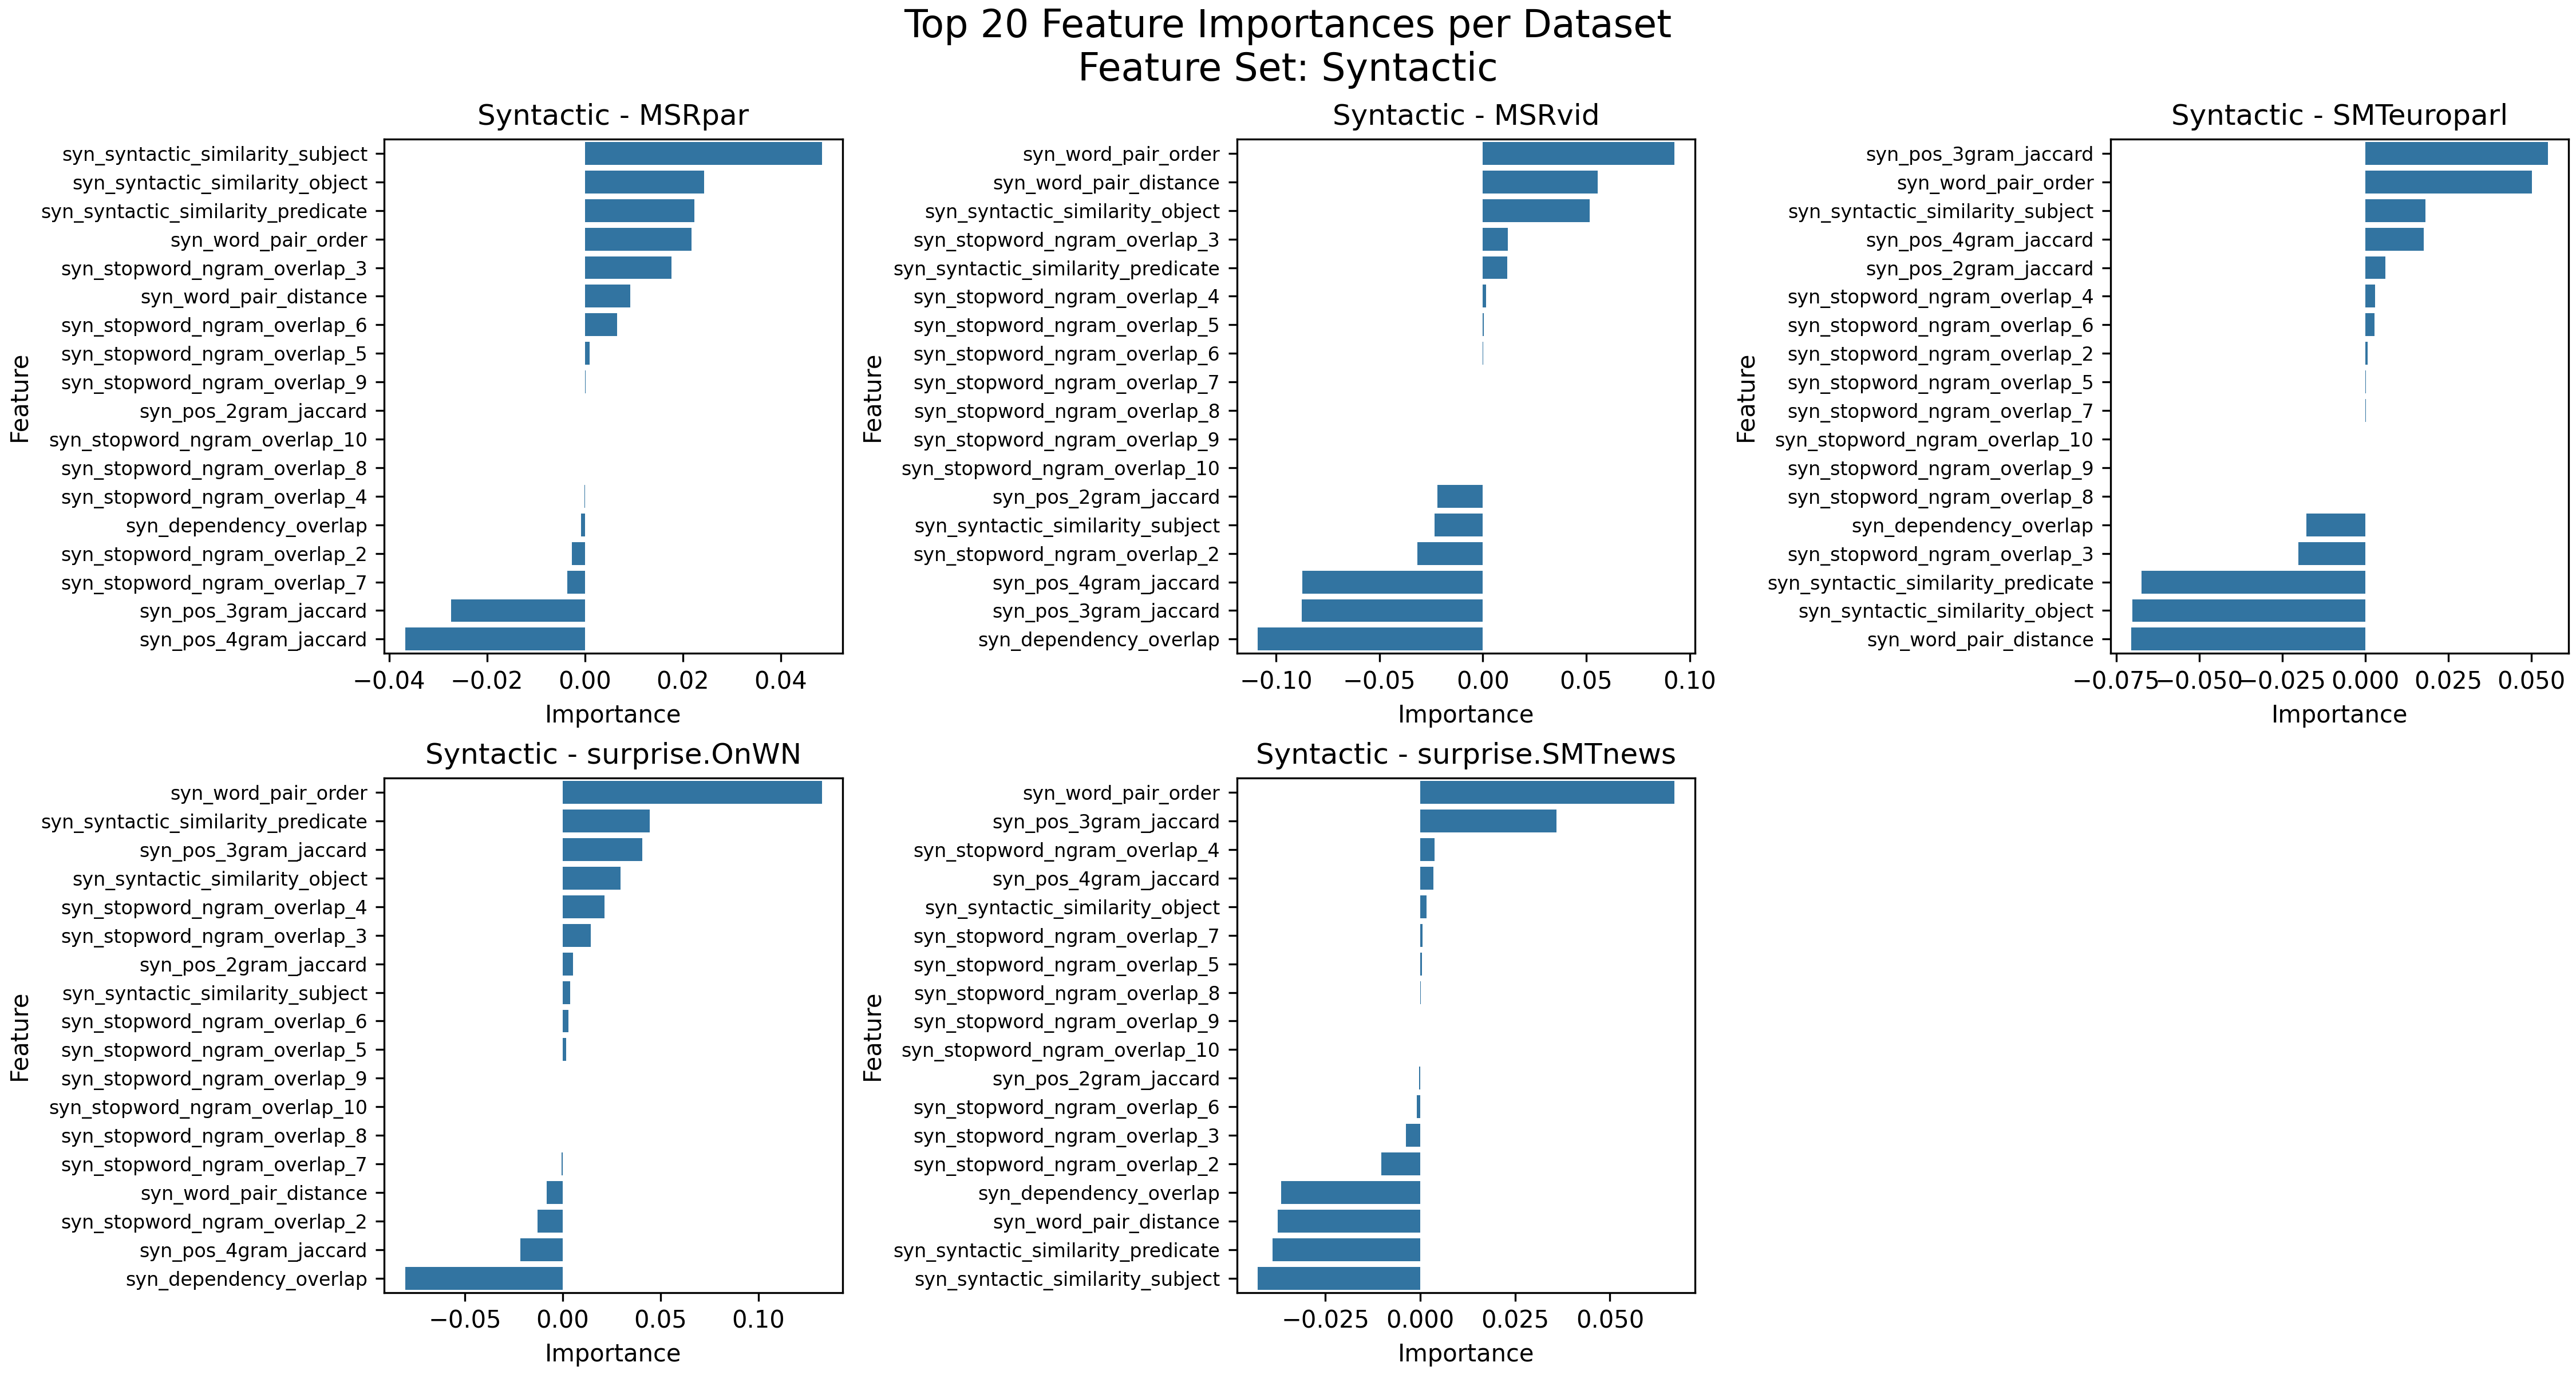
\includegraphics[width=0.9\linewidth]{img/FI_dataset_Syntactic.png}
    \caption{Feature Importance per Dataset, Syntactic Model}
  \end{figure}
  \centering
  \textit{Feature importance heavily depends on the dataset.}

  \begin{figure}
    \centering
    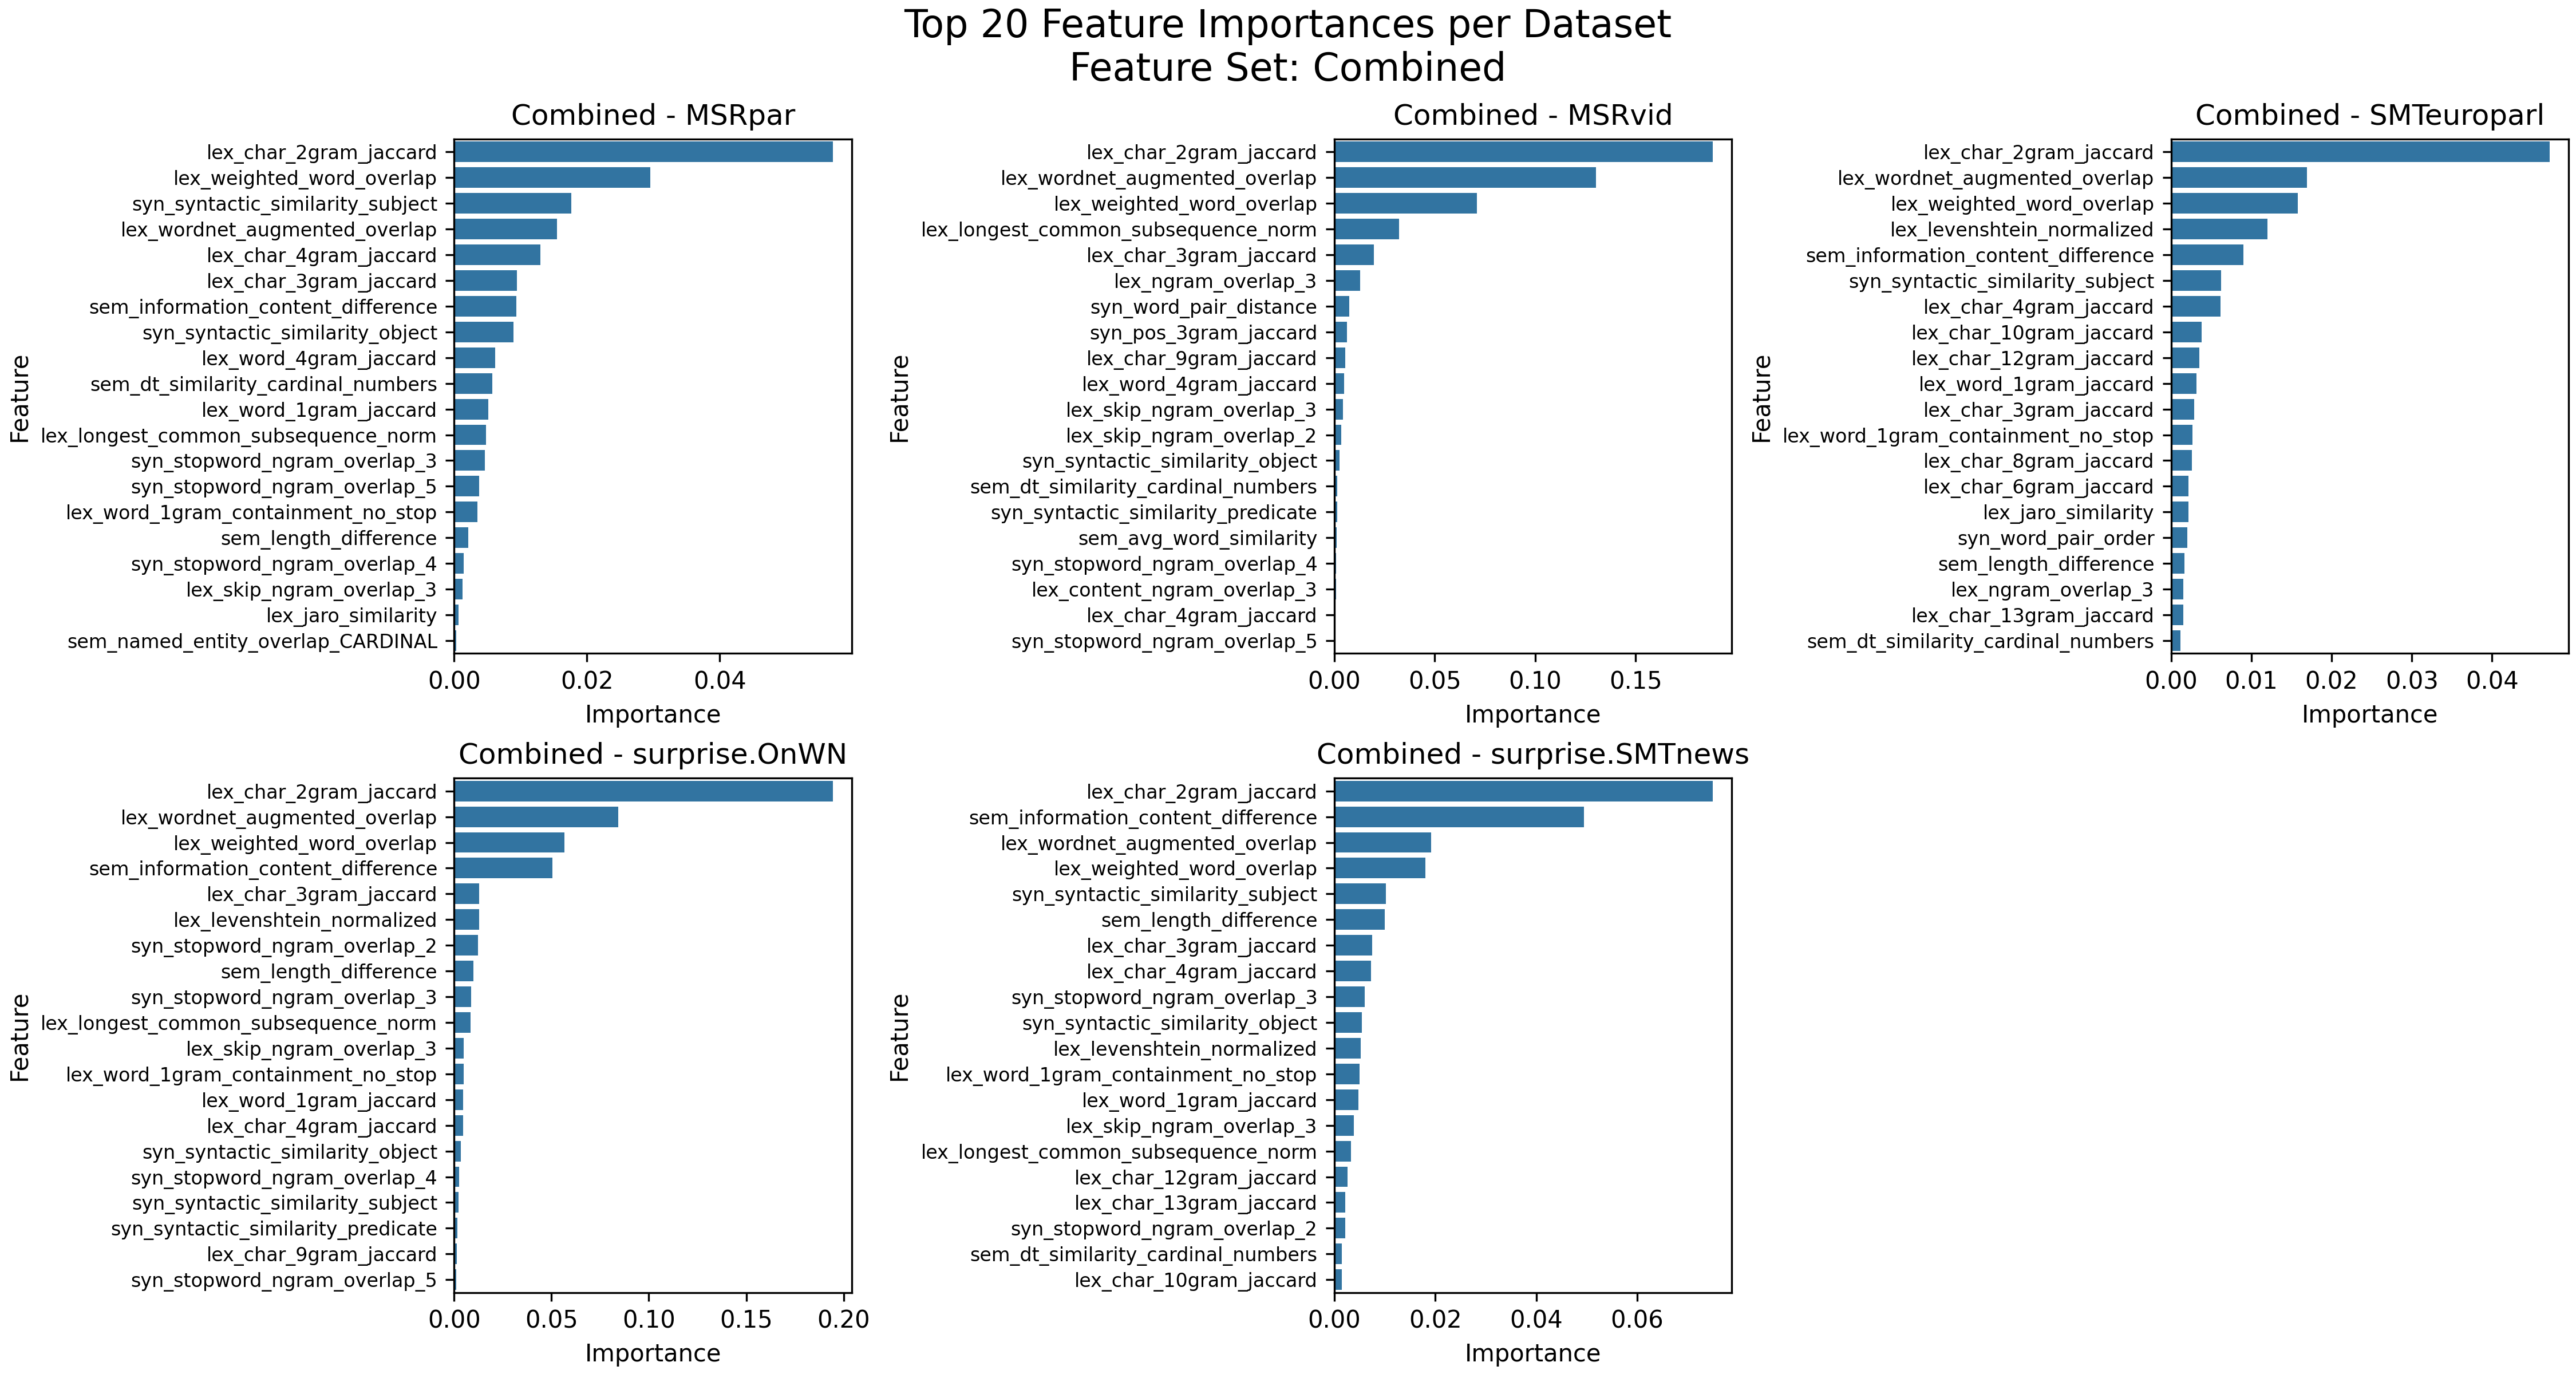
\includegraphics[width=\linewidth]{img/FI_dataset_Combined.png}
    \caption{Feature Importance per Dataset, Combined Model}
  \end{figure}
  \centering
\end{frame}

\section{Error Analysis}

% Slide 15: Distribution of Errors
\begin{frame}
  \frametitle{11. Error Analysis - Density and Predictions}
  \begin{itemize}
    \item Observed a tendency to \textbf{overpredict} similarity scores.
    \item \textbf{Reason:} Optimizing for Pearson $\rightarrow$ \textbf{Metric Exploitation.}
  \end{itemize}
  \begin{figure}
    \centering
    \begin{minipage}{0.42\linewidth}
      \centering
      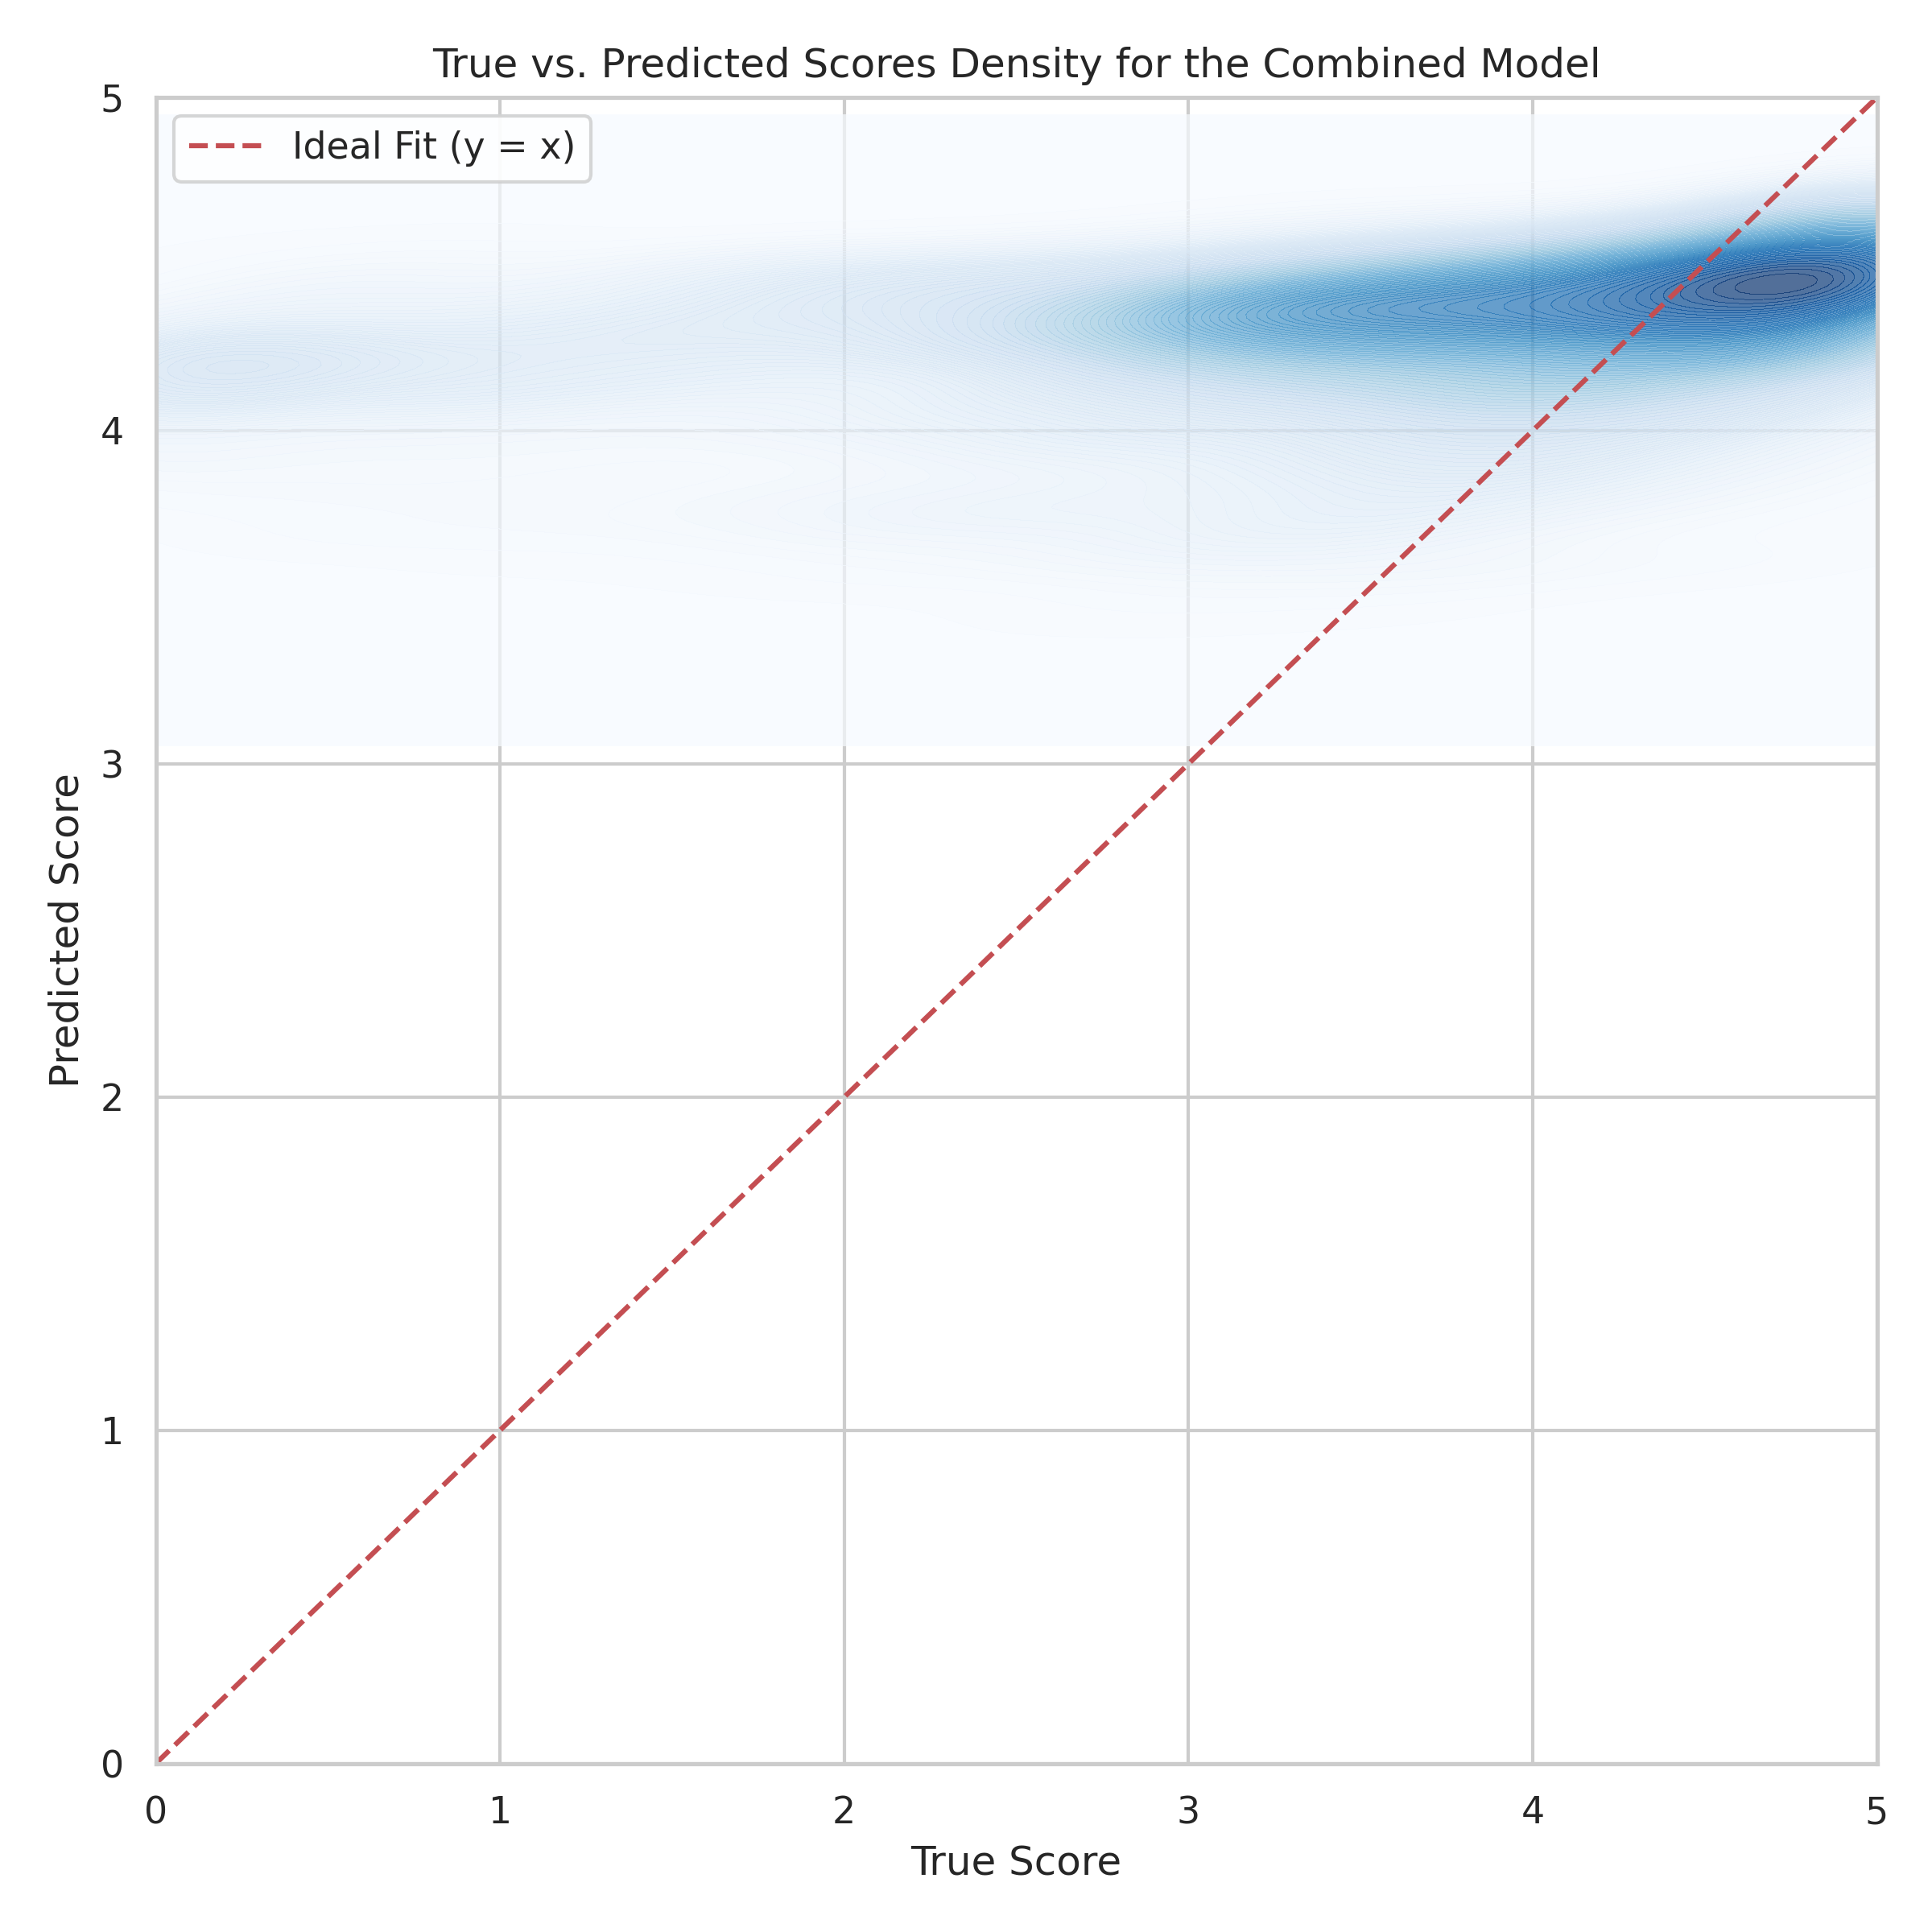
\includegraphics[width=\linewidth]{img/density_true_vs_combined.png}
      \caption{True vs Combined, Density}
    \end{minipage}
    \hfill
    \begin{minipage}{0.5\linewidth}
      \centering
      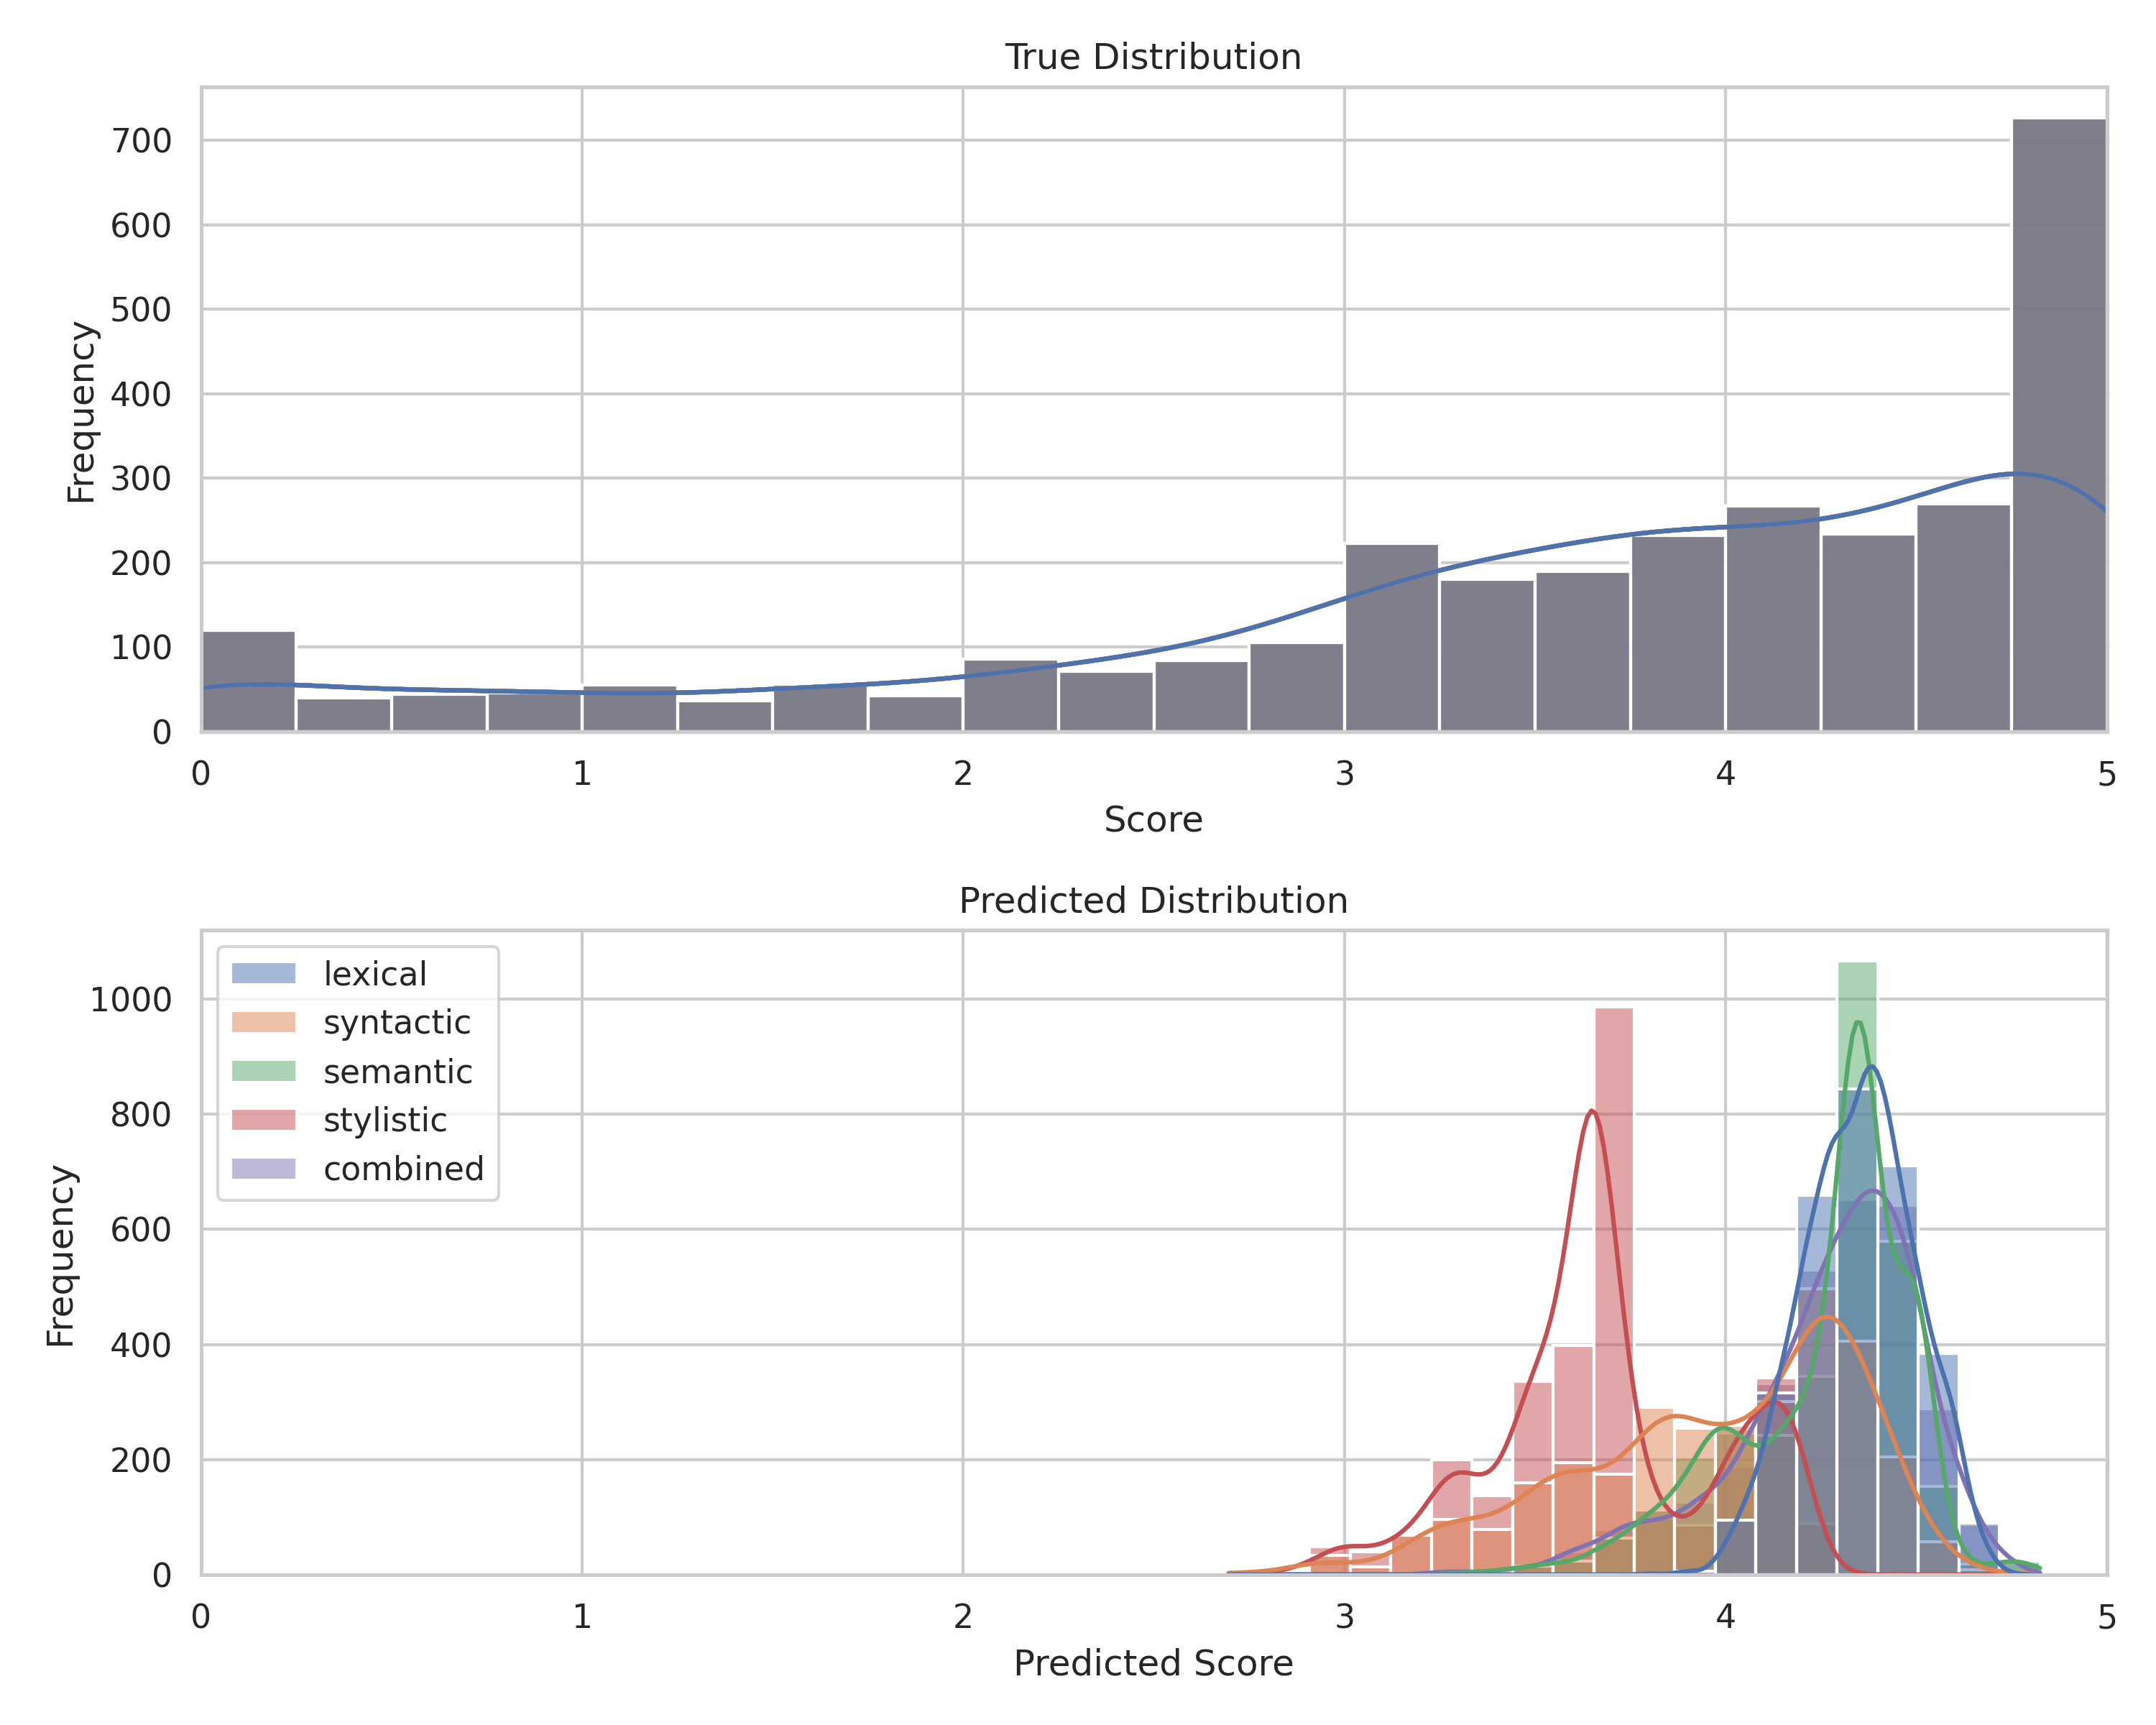
\includegraphics[width=\linewidth]{img/true_vs_pred_dist.png}
      \caption{True and Predicted Distribution}
    \end{minipage}
  \end{figure}
\end{frame}


\section{Summary and Conclusions}

% Slide 16: Summary and Conclusions
\begin{frame}[allowframebreaks]
  \frametitle{11. Summary and Conclusions}
  \begin{itemize}
    \item \textbf{Project Overview:}
    \begin{itemize}
      \item Implemented STS using features inspired by UKP\cite{bar-etal-2012-ukp} and TakeLab\cite{saric-etal-2012-takelab} (SemEval 2012 Task 6).
      \item Evaluated the impact of \textbf{lexical}, \textbf{syntactic}, \textbf{semantic}, and \textbf{stylistic} features.
    \end{itemize}
    \vspace{0.3cm}
    \item \textbf{Key Results:}
    \begin{itemize}
      \item Combined feature set achieved a Pearson correlation of \textbf{0.7634}, \textbf{top 10} in a simulated ranking.
      \item \textbf{Top 1} in mean Pearson: consistently performed well across all datasets
      \item \textbf{Lexical features} were most influential, especially in datasets with high word overlap.
      \item \textbf{Syntactic and semantic features} improved performance on datasets with complex structures or varied wording.
      \item \textbf{Stylistic features} had minimal impact on similarity scores.
    \end{itemize}
    \vspace{20cm}
    \item \textbf{Challenges Faced:}
    \begin{itemize}
      \item Resource and computational constraints led to approximations in feature implementations.
      \item Tool differences may have affected performance compared to original teams.
      \item Reliance on Pearson correlation may have encouraged overprediction.
    \end{itemize}
    \vspace{0.3cm}
    \item \textbf{Future Work:}
    \begin{itemize}
      \item Refine feature implementations (e.g., full-scale ESA, advanced skip n-grams).
      \item Perform a better feature selection
      \item Address overprediction (adjusting evaluation metrics, employing calibration techniques, ...)
    \end{itemize}
  \end{itemize}
\end{frame}

% Slide 15: Ending Slide
\begin{frame}
% \frametitle{13. Thank You}
\begin{center}
\Huge\textbf{Thank You!}
\vspace{1cm}


\Large Questions?
\end{center}
\end{frame}

\begin{frame}[allowframebreaks]{References}

\bibliography{references}

\end{frame}

\end{document}
